\documentclass[10pt,a4paper]{ULBreport}
\usepackage[utf8]{inputenc}
\sceau{pic/official_logos/sceauULB.png}
\graphicspath{ {./pic/} }
\usepackage{multirow}
\usepackage{listings}
\usepackage{color} 
\usepackage{setspace} 
\usepackage{amsmath}
\usepackage{hyperref}
\usepackage{pdfpages}
\usepackage{biblatex}
\usepackage{floatrow}
\usepackage{subcaption} 
\usepackage{siunitx}
\usepackage[many]{tcolorbox}
\usepackage{multirow}
\usepackage{listings}
\usepackage[dvipsnames]{xcolor}
\usepackage{fancyvrb}

\usepackage{xstring}
\usepackage{etoolbox}

% Colors



\begin{document} 


	\titleULB{
	title={CmOS},
    studies={MA1-IRELE},
    course ={OS and security},
    author={\textit{Author :} \\ Emmeran Colot },
    date={\textbf{Academic year :} \\ 2024 - 2025},
    teacher={\textit{Professor : } \\ Prof. B. Da Silva},
    logo={pic/official_logos/logos.jpg},
    manyAuthor
	}

%\listoftables % ToC for tables

%\listoffigures % ToC for figures

\chapter{Introduction}

In this report, a comparison of two ways of storing files is made. There is a main focus on how those storage systems work, followed by a comparison of their performance. \\

The project was initially named \textit{CmOS} for \textit{C modeled OS} as it was supposed to implement more than only a storage system. The whole code is available on github\footnote{\href{https://github.com/e-colot/CmOS}{https://github.com/e-colot/CmOS}} and one can see that the basic building blocks for a complete OS are present. It includes registers definition, a custom ISA, a compiler and an interpreter for going from assembly to binary and then execute it and so on, but they will not be discussed as the project objective has changed to the study of storage systems. It is a smaller topic but there is still a lot to say about it. 

Finally, there are a few remarks:
\begin{itemize}
    \item This whole project has been built by hand with no external source. This means that the two systems are not based on any existing system but only on the knowledge acquired during the course and on some personal ideas.
    \item In the following, the terms \textit{file system} and \textit{storage system} will be used interchangeably
    \item Except when specifically mentioned, the term \textit{disk} will refer to the simulated disk.
\end{itemize}






\chapter{Background}

As everything is built from scratch, there is not a lot of prerequisite knowledge needed to understand this report. However, a few concepts are important to understand how the two systems work.

\section{disk}
\label{sec:disk}

The disk is where files are stored on a computer and it can be seen as a big vector of bytes. To read or write some data, an address is given and the driver will read or write the data at that address. A real disk will often have different sectors with a longer access time when changing sectors. \\

In the simulation, the disk is a file on the computer of which the size is fixed by a parameter. Because of this, there is no access time when changing sectors. However, because of paging (which will be explained later) and depending on the computer on which the simulation is run, the access time could indeed be longer when reading or writing data at addresses that are far away from each other but this is, once again, outside of the scope of this analysis. \\

\section{Paging}
\label{sec:paging}

When storing data in memory, it would be inefficient to have data blocks of varying sizes. This is why the memory is divided into blocks of fixed size. Each of those blocks is called a \textit{page} and the size of a page is called the \textbf{page size}. This size will be an important parameter in the following.

\section{File system}
\label{sec:filesystem}

The file system is in charge of managing the data on the disk. It is responsible for writing files, accessing written files and deleting them. It might have additional features but those are sufficient for a working file system and the one built here only implement those basic operations.







\chapter{Description of the storage systems}

\section{generalities}
\subsection{Variable page size}
As described in section \ref{sec:paging}, both file systems will use paging to store data. The page size is variable and can be set when creating the file system. Building a variable page size system is not a difficult task unless it aims to be efficient. Both of the systems built here have been designed to be efficient so this single feature has doubled the development time.
\subsection{Folders}
For the sake of simplicity, the two systems will not implement folders. This is a choice that is often made for small size operating systems such as for RTOS\footnote{Real Time Operating System}.
\subsection{Addressing bytes}
The disk is split into pages of a fixed size but when trying to write or read a page, there must be a way of pointing to it. Because the disk size and the page size are parameters, one can not assume a single byte address will be enough to address all the pages. \\
A disk of 256 kB with a page size of 256 bytes will have 1024 pages and a single byte address can only go up to 255. This means that a single byte address will not be enough to address all the pages. This is why the number of bytes used to address a page, referred to as \textbf{addressing bytes} or $A_b$, is variable and is computed as follows:
\begin{equation*}
    A_b = \lceil \log_2\left(\frac{\text{disk size}}{\text{page size}}\right) \rceil
\end{equation*}
The complexity of addressing with a variable number of bytes is that, depending on the dimensions of the disk and the page size, the place needed to store an address can vary, making the disk content vary. As the disk is only a file on the computer running the simulation, it is limited in size so more than 4 addressing bytes are not implemented. This would correspond to a disk of 64 GB with a page size of 16 bytes\footnote{This value of 16 bytes is not chosen randomly, it will be explained later.}.
\subsection{File allocation table}
Somewhere on the disk, there is a space reserved for the file allocation table (FAT). This table is used to store the information about the files on the disk. All the information related to a file will be referred to as an \textit{entry} or a \textit{file entry}.\\
It stores at least the following information:
\begin{itemize}
    \item A way to uniquely identify the file
    \item The address of the first page of the file
\end{itemize}
and it can store more information, as will be shown later in one of the systems.
\subsection{File identifier}
The file identifier is, as described in the previous section, a way to uniquely identify a file. It is generally a string of characters, corresponding to the name of the file. Because this simulation aims to be efficient and it can work with a really small disk (most of the tests were done with a 4kB disk), having a string would quickly fill the disk. \\
For this reason, the file identifier is simply a number. This number is different of zero, which is a reserved number for an empty file. To make sure that every file is can have a unique identifier, this \textbf{ID} is stored on the same number of bytes as the addressing bytes. As each file is stored on at least one page, which address holds on $A_b$ bytes, using the same number of bytes for the ID will be enough to store the ID of the file. \\
When adding a file, the given ID is checked against the IDs found in the FAT to avoid duplicates and an error mechanism is implemented to handle this case. 
\subsection{File terminator}
Because the files are stored in pages, there often are bytes at the end that are not data. Because only the number of pages used to store the data is known (and not the number of bytes), there is a need to differentiate the bytes that compose the data and the ones that are not and this is the interest of having a file terminator. \\
At the end of the file, \texttt{0x00} is added and this is the file terminator symbol. It is then followed by a padding: the rest of the page is filled with \texttt{0xFF}. If this padding was not made, there could be a risk of having another \texttt{0x00} that would be interpreted as the terminator.

\section{Linked list allocation system}
\label{sec:linkedlist}
\subsection{Description}
The first system is a linked list allocation system. This means that the pages of a file are not stored next to each other on the disk. Instead, each page contains at its beginning a pointer to the next page of the file. The last page has a pointer to zero, indicating that it is the last page of the file.
\subsection{Bitmap}
Because the pages are not stored next to each other, there is a need for a way to know which pages are free to be used and which ones are already used. It is for this reason that a bitmap is present at the beginning of the disk. \\
Each bit of the bitmap corresponds to a page on the disk and is set to 1 if the page is used and to 0 if it is free.
\subsection{FAT structure}
The first FAT page is always placed right after the bitmap. As more files are added, the FAT will grow and at some point, a single page will not be enough. The next page is then chosen among the free pages (found in the bitmap) and the previous page will point to the new page. This allows the FAT to grow as needed and make this system scalable. 
\begin{figure}[H]
    \floatbox[{\capbeside\thisfloatsetup{capbesideposition={right,top},capbesidewidth=0.5\textwidth}}]{figure}[\FBwidth]
    {\caption{The structure of the File Allocation Table (FAT) in the linked list allocation system.\\ It starts with $2 A_b$ bytes linking to the previous and the next FAT pages. It is then followed by \textit{entries} of $2 A_b$ each with the ID of the file and the address of the first page where the file is written.\\ Because each little box on the figure contains $A_b$ bytes and because $A_b$ is not bigger than 4, a page size smaller than 16 could lead to issues. In the case of a page size of 15 and $A_b = 4$ (with a huge disk size for instance), the first row will already use 8 out of the 15 bytes. There will then not be enough bytes left to write a single file entry in the page, making it useless}\label{fig:FAT_LL}}
    {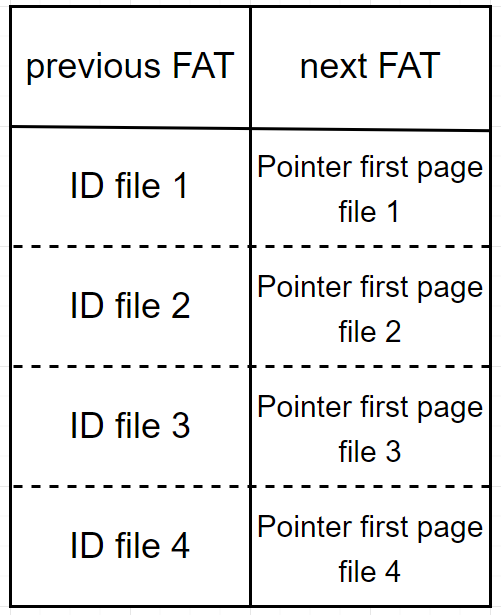
\includegraphics[width=0.4\textwidth]{FAT_LL.png}}
\end{figure}
\subsection{Finding a free page}
For writing operations, there is often the need to find a page that is not used. Because the files must not be stored one after the other, the address returned is purely random, but it still must be an unused one. The first approach that was implemented was a \textit{Random Access} method:
\begin{enumerate}
    \item Take a random address < number of pages
    \item If it is already used, go back to \textbf{1.}
    \item If not, return the address
\end{enumerate}
It has been replaced later on by the \textit{Continue Until Found} method:
\begin{enumerate}
    \item Take a random address < number of pages
    \item If it is already used, check the next address and go to \textbf{2.}
    \item If not, return the address
\end{enumerate}
To compare the two approaches for finding a free page, a simulation was run where the disk was gradually filled, and the time taken to find a free page was recorded. The results are shown in Figure \ref{fig:findFreePageTime}. \\
\begin{figure}
    \centering
    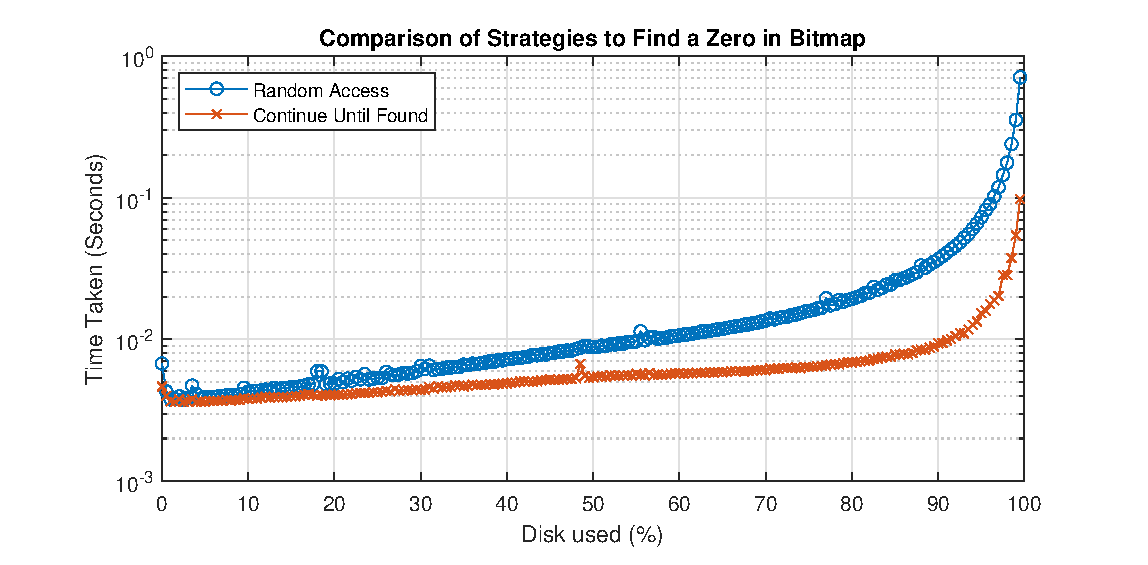
\includegraphics[width=1\textwidth]{findFreePage.eps}
    \caption{Comparison of the time taken to find a free page as the disk fills up. This simulation was done with a toy script in Matlab, not the real system}
    \label{fig:findFreePageTime}
\end{figure}
The second approach, which checks the next address sequentially, performs significantly better when the disk is nearly full, which was expected as it has the certitude of finding a free page after having searched through the whole bitmap.
\subsection{Adding a file}
A simplified version of the algorithm to add a file is shown on the logical diagram \ref{fig:Logic_add_LL}. There are a lot of checks to be done when adding a file and those are not included in the diagram. \\
For instance, if no page new page is found for writing after the file entry has been put in the FAT (inside the while loop in \ref{fig:Logic_add_LL}), it means that the disk is full. However, as the file is not entirely written, it cannot stay there as it could potentially be read and it would not be the same data as what was given. The fix for it is to mark the last page as the end of the file with a pointer to 0 (see the next section to understand why it is important) and then remove the file.
\begin{figure}
    \centering
    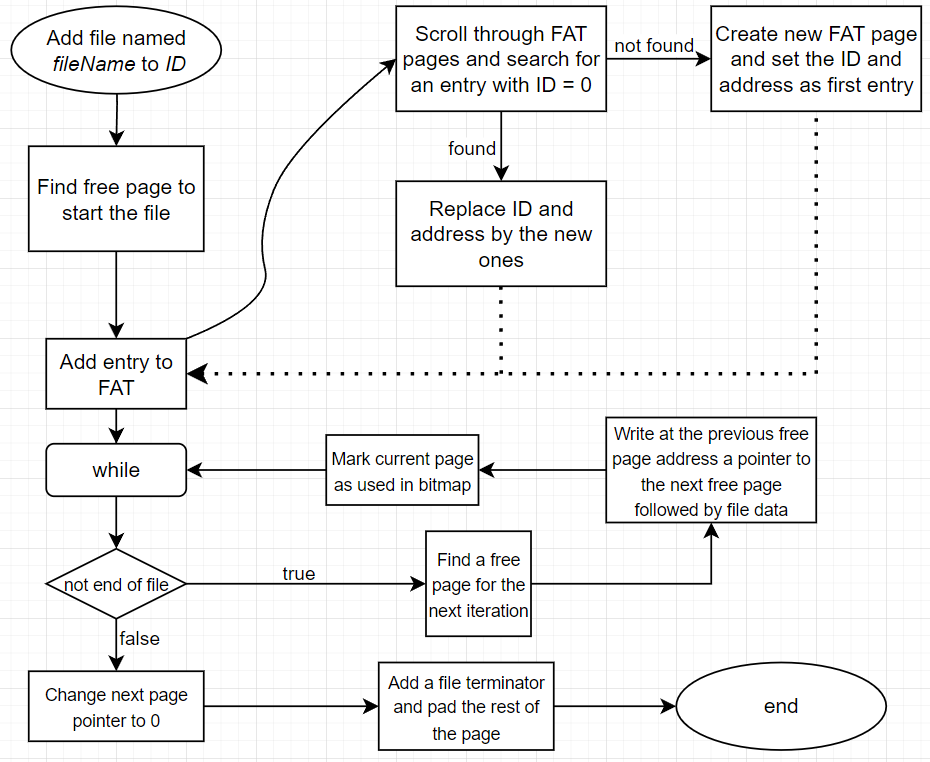
\includegraphics[width=0.8\textwidth]{Logic_add_LL.png}
    \caption{Logical diagram of the algorithm to add a file in the linked list allocation system}
    \label{fig:Logic_add_LL}
\end{figure}
\subsection{Removing a file}
To remove a file, its entry must be removed from the FAT and all the pages used to store the file must be cleared in the bitmap. Removing the entry is straightforward: it cycles through the FAT pages and search for the ID. When found, it sets the ID to 0 to indicate that there is no more file\footnote{This is the reason why the ID 0 cannot be used by any file} and the address of the first page is stored. From there, it sets the current page as free in the bitmap and load the next page of the file (using the pointer at the start of the current page) until the next address is 0, which indicates the end of the file.
\subsection{Loading a file}
There is not much to say about this. It proceeds like for a page removal except that instead of marking the page free in the bitmap, it gets rid of the pointer to the next page and load the data in a buffer to be sent back.
\subsection{FAT reorganization}
Once in 10 times a file is removed, a FAT reorganization takes place. It will fill the holes in the first FAT pages (entries with ID = 0) with entries that are in the last pages of the FAT. This allows to empty the last FAT pages and to remove them. It frees some pages which can then be used to store more files.

\section{Contiguous allocation system}
\label{sec:contiguous}
\subsection{Description}
The second system is a contiguous allocation system. This means that the pages of a file are stored next to each other on the disk. This is a simpler system but it still needs some work to be done to make it efficient. \\
The FAT will be stored in the first pages of the disk and the files will be stored starting from the end of the disk. This way, the FAT can grow as needed and the disk will be considered as full when adding a file will make its first page collide with the FAT.
\subsection{FAT structure}
\label{sec:FAT_CA}
Unlike the linked list allocation system, the FAT is not a linked list. It starts at 0 and then grows as needed. It will not be restrained to pages. This means that a file entry might be between two pages.\\
Because the files are stored on adjacent pages, there is no way to know where the file stops. This is why a FAT entry will contain, additionally to the ID and the address of the first page, the size of the file in pages. This way, when loading a file, the system will know how many pages to load. \\
A FAT entry will be structured as follows:
\begin{figure}[H]
    \centering
    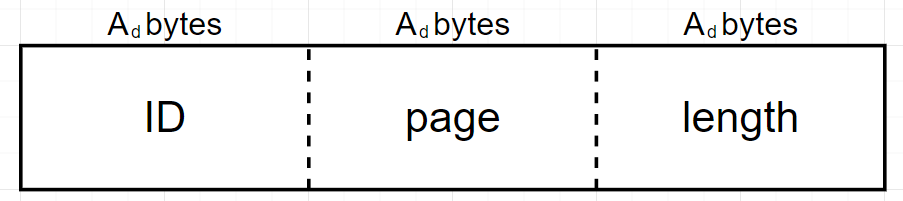
\includegraphics[width=0.6\textwidth]{FAT_entry_CA.png}
    \caption{The structure of a FAT entry in the contiguous allocation system.}
    \label{fig:FAT_C}
\end{figure}
The first FAT entry will be referred to as the \textit{FAT info}. It contains 0 in its ID field, the page stores the number of pages used by the FAT and length will be the number of entries in the FAT. \\
After the FAT info, the entries are stored in reverse order relative to their placement on the disk. This means that the first entry in the FAT corresponds to the file placed at the end of the disk, and subsequent entries follow in reverse order of their placement. Maintaining this order is crucial and it is the reason why a contiguous allocation system is not much easier to implement than a linked list allocation system.\\
\subsection{Adding a file}
The algorithm to add a file is quite different from the one used in the linked list allocation system. A simplified version of the algorithm to add a file is shown on the logical diagram \ref{fig:Logic_add_CA}.\\
\begin{figure}
    \centering
    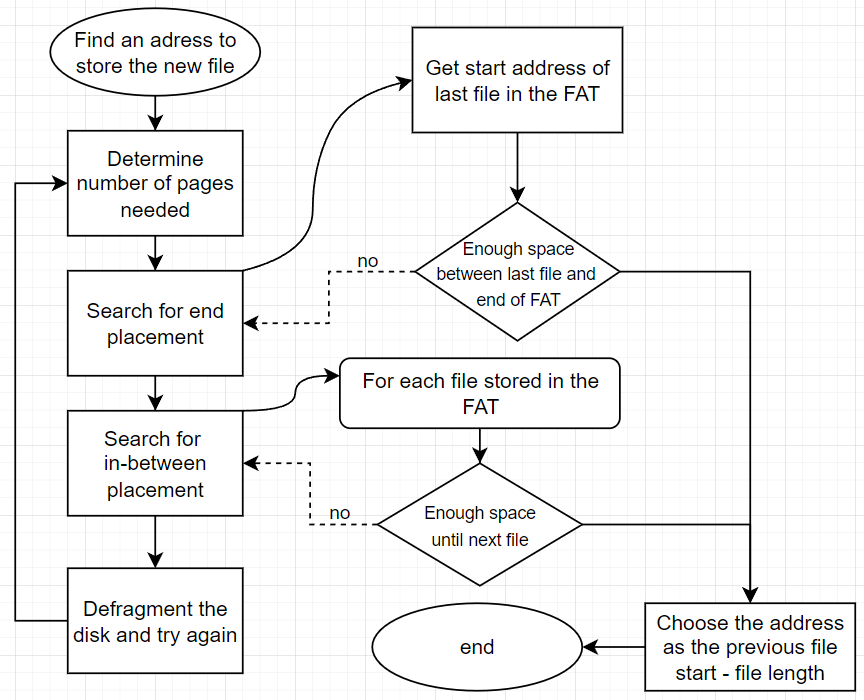
\includegraphics[width=0.8\textwidth]{Logic_add_CA.png}
    \caption{Logical diagram of the algorithm to add a file in the contiguous allocation system}
    \label{fig:Logic_add_CA}
\end{figure}
The disk defragmentation will be detailed in a later section but it allows to make more space available on the disk. The \textit{in-between} check is to see if the file can be added between two files.  
One among the checks that is not shown in the diagram is for instance the check to see if adding the file will not make the FAT collide with it. Just finding the number of pages that are used by the FAT is a quite complex task. Even if the file fits between the last file and the FAT, it could be that adding the entry will make the FAT grow and then collide with the file. It might be a bit tricky so the figure \ref{fig:FAT_collision} shows in 3 steps how such issue could arise. \\
\begin{figure}
    \centering
    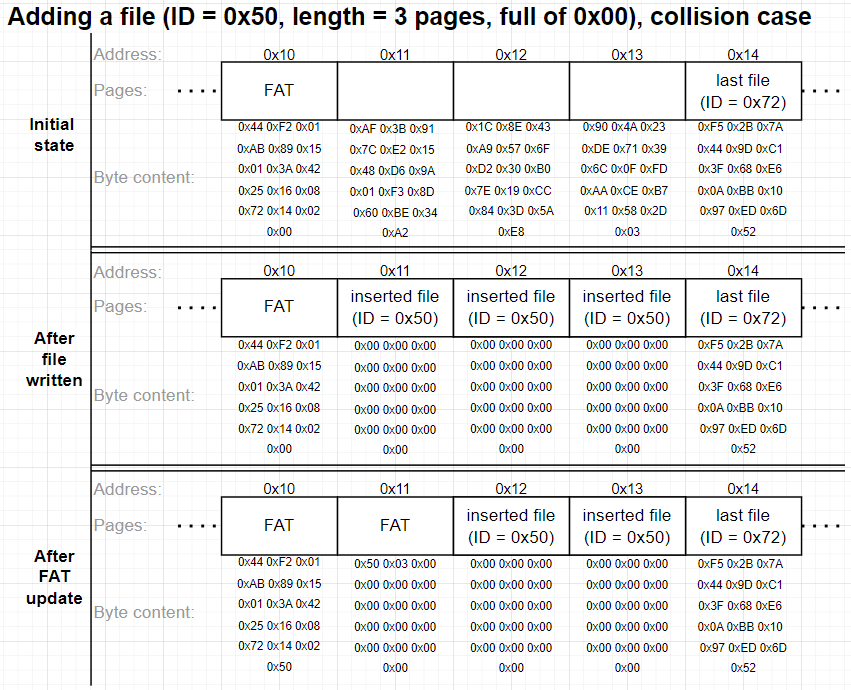
\includegraphics[width=0.8\textwidth]{FAT_collision_CA.png}
    \caption{Example of a collision between the FAT and a file. The page size is set to 16 bytes. It also shows how a FAT entry can be between two pages.}
    \label{fig:FAT_collision}
\end{figure}
\subsection{Removing a file}
As per the linked list allocation system, removing a file is simply done by removing the entry from the FAT. Because there is no bitmap, there is no need to go through the pages of the file but the FAT must be reorganized once the entry is removed. \\
Every entry from the previous entry location to the end of the FAT must be shifted to lower addresses. This is indeed needed to keep an ordered FAT as detailed in section \ref{sec:FAT_CA}. 
\subsection{Loading a file}
Loading a file is done by reading the entry in the FAT and loading the pages that are needed. The number of pages to load is stored in the entry so it is straightforward.
\subsection{Disk defragmentation}
In two scenarios, no file can be added to the disk if no defragmentation is done:
\begin{figure}[H]
    \centering
    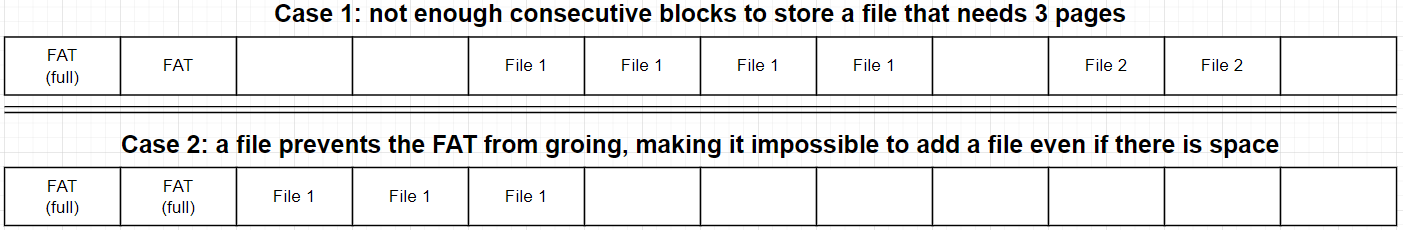
\includegraphics[width=1\textwidth]{Reason_for_fragmentation_CA.png}
    \caption{Examples of a non full disk that cannot accept a file until the disk is defragmented. }
    \label{fig:defrag}
\end{figure}
The objective of the disk defragmentation is to remove any gaps between files on the disk and to put the files back to the end of the disk to make space for the FAT. The algorithm is quite simple:
\begin{enumerate}
    \item Start from the first entry in the FAT and use as last page the end of the disk
    \item If the end of the actual file is before the last page, move the file to the end of the disk and update the FAT entry with the new address
    \item Repeat \textbf{2.} for the next file
\end{enumerate}
This process is the equivalent of the \textit{FAT reorganization} in the linked list allocation system. As it is a way of cleaning the disk. The difference is that the FAT reorganization is a lighter process and even if not done, the system will work fine whereas with no defragmentation, the second scenario in figure \ref{fig:defrag} will brick the system until \textit{File 1} is removed. \\








\chapter{Testing the systems}
Both systems have been tested in multiple cases. As the way of addressing changes depending on the disk size and the page size, tests have been done with different combinations of those two parameters to see how the systems behave for all the possible addressing bytes values.\\
The test scenario is as follow:
\begin{itemize}
    \item A few files are created on the computer running the simulation with different sizes
    \item A random number of files chosen randomly in the test files are added to the disk
    \item A random number of files are removed from the disk
    \item All files on disk are compared with the initial files
    \item The disk is filled with files
    \item The files are checked
    \item A random number of files are removed
    \item A random number of files are added one more time
    \item All files are checked again
\end{itemize}
To check the stored files, the computer simulating the file systems stores what ID's are given to which file. The ID of the files that have been stored are compared with the ones in the FAT to make sure every file is stored and no removed file is left in the FAT. The data integrity is also checked by comparing the first, the last and 10 randomly placed bytes between the original file and the one stored by the simulation.












\chapter{Experimental results}
Two experiments have been done to compare the two systems. Every measurement has been done 50 times and xas then averaged. This is because the experiments include some randomness which could lead to different results. \\
Both of the experiments have been done with a disk size of 16kB and a page size varying from 16 bytes to 512 bytes. The operations used are similar to the ones made during the tests:
\begin{itemize}
    \item Adding a random number of files
    \item Removing a random number of files
    \item Filling the disk with files
    \item Emptying the disk
\end{itemize}
\section{Experiment 1}
\subsection{Description}
The first experiment is to fill the disk with files and then empty it. The time taken to fill the disk and the time taken to empty it are measured. The results are shown in figure \ref{fig:fillDisk} and \ref{fig:emptyDisk}. \\
\begin{figure}
    \centering
    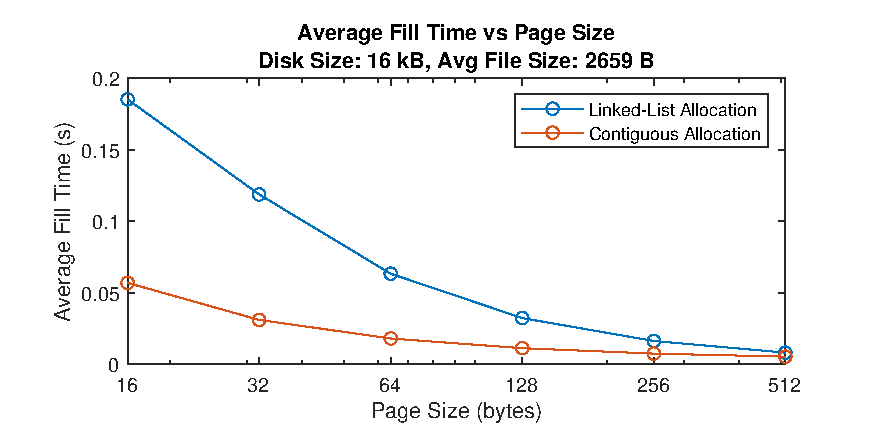
\includegraphics[width=1\textwidth]{FillDisk.eps}
    \caption{Time taken to fill the disk with files. The time is in seconds and the page size is in bytes.}
    \label{fig:fillDisk}
\end{figure}
\begin{figure}
    \centering
    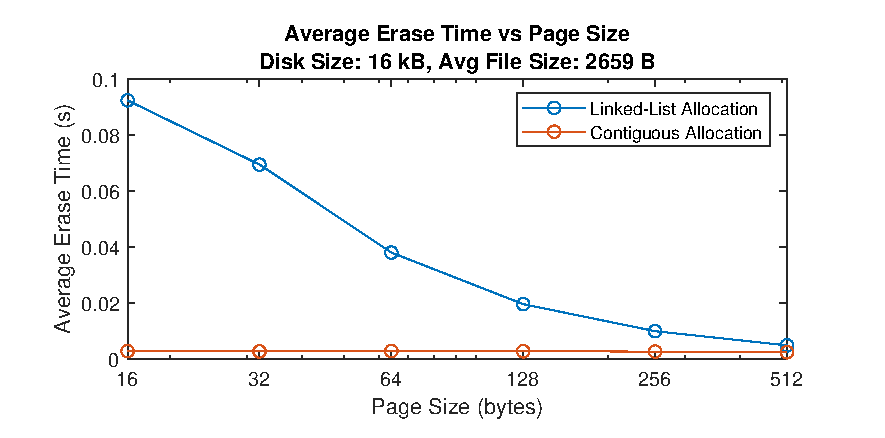
\includegraphics[width=1\textwidth]{EraseDisk.eps}
    \caption{Time taken to empty the disk. The time is in seconds and the page size is in bytes.}
    \label{fig:emptyDisk}
\end{figure}
\subsection{Interpretation of the results}
The first experiment shows that both for filling and emptying the disk, the contiguous allocation system is 3 times faster than the linked list allocation system for a small page size. This is easily explained by the fact that the linked list allocation system has to go through the bitmap to find a free page and then write the pointer to the next page in the file. \\
However, as the page size increases, the performance of the two systems becomes similar. Indeed, if the file fits in a single page, the contiguous allocation system will not be much faster than the linked list allocation system. \\
\textbf{Note: } The time taken to fill the disk in a contiguous allocation system should be constant as the files are stored one after the other. It is, however, not the case and this is probably due to the fact that to store data from the simulating computer to the disk, the data is copied in a buffer and then written to the disk. This buffer was chosen to have the same size as the page size. This means that when the page size is small, the buffer is small and the time taken to write it to the disk is longer. \\
Concerning the erasing time, The contiguous allocation system is also the fastest and the time needed to erase the disk is almost constant. This is because removing a file is done by removing the entry in the FAT. \\
It is a much complex task for the linked list allocation system as it has to go through the pages of the file to mark them as free in the bitmap. This is why the time taken to erase the disk is not constant and decreases with the page size as a single file will take less pages. \\
\section{Experiment 2}
\subsection{Description}
The second experiment aims to measure the writing data rate and the disk usage depending on the page size. This is done by first filling the disk and then removing a few of them. The disk is then filled again and the time taken to achieve this is measured. The results are shown in figure \ref{fig:normalOP}. \\
To determine the disk usage, the number of bytes coming from files stored on the disk is divided by the capacity of the disk. This allows to avoid taking into account the bytes written by the storage system itself such as FAT pages, pointers for linked list allocation system, etc. \\
\begin{figure}
    \centering
    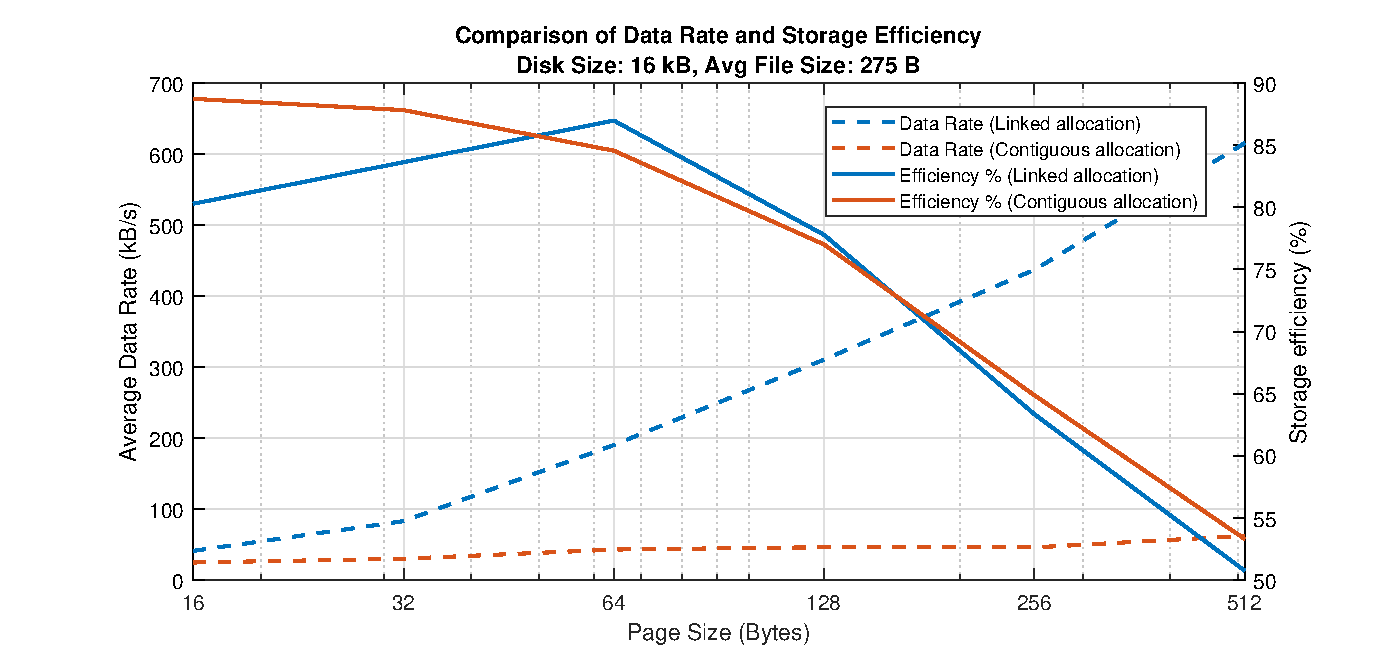
\includegraphics[width=1\textwidth]{normalConditions.eps}
    \caption{Writing data rate (dashed lines) and disk usage (solid lines) depending on the page size}
    \label{fig:normalOP}
\end{figure}
\section{Interpretation of the results}
The results of figure \ref{fig:normalOP} show values for a realistic use of the system. The previous experiment was advantaging the contiguous allocation system because the first fill of the disk will result in files being stored one after the other. This is not the case in this experiment as files are removed in between. This means the defragmentation process, which was heavy, will be used. This new test setup has no impact on the performance of the linked list allocation system.\\
The linked list allocation system sees an increase in the writing data rate as the page size increases. As explained in the previous section, a single file will take less pages and the time taken to write it to the disk is shorter. The contiguous allocation system, on the other hand, sees close to no increase in the writing data rate. This is because, no matter the page size, every file that is added first needs to check if it can be added between two files and will then call the defragmentation process. Those two operations are not depending on the page size but on the number of files on the disk. \\
The disk usage is quite similar for both systems. It sees a decease when the page size increases. This is because the number of pages used to store a file must be an integer and every byte that is not used in the last page is wasted. An interesting point is that the disk usage of linked list allocation starts $5\%$ lower than the contiguous allocation before joining it around a page size of 64 bytes. This is because for every page, the linked list allocation system has to store a pointer to the next page and this wasted space will be heavily depending on the number of pages used. A more significant difference was expected for a page size of 16 bytes as the number of addressing bytes is 2 in this case, doubling the number of bytes used for every single pointer. \\
The following calculations can convince anyone that the disk usage of the linked list system can never beat the one of the contiguous allocation system (except when the sizes of the files are convenient):
\begin{itemize}
    \item Because the average file size is 275 bytes, an average file will need $275/14 = 13$\footnote{14 instead of 16 as 2 bytes of the page will be used to point to the next page} pages which results in $30$ bytes wasted per file (taking the file entry in the FAT into account).
    \item The same file stored in a contiguous allocation system would only need $6$ bytes: 2 for the ID, 2 for the page address and 2 for the length, which is by far more optimal. 
\end{itemize}










\chapter{Conclusion}
This concludes this study of file systems. It showed that both systems have their own strength, which are show in the following table.

\begin{table}[H]
    \centering
    \begin{tabular}{|l|p{5cm}|p{5cm}|}
        \hline
        \textbf{Criteria} & \textbf{Linked List Allocation} & \textbf{Contiguous Allocation} \\ \hline
        \textbf{Write speed at low disk usage} & 
        slow due to linking process & 
        fast because of end placement \\ \hline
        \textbf{Write speed at high disk usage} & 
        faster & 
        slower due to disk defragmentation \\ \hline
        \textbf{Disk efficiency} & 
        slightly lower because of the high number of pointers but similar performances for higher page sizes & 
        as high as a system using paging could get \\ \hline
    \end{tabular}
    \caption{Comparison of Linked List Allocation and Contiguous Allocation File Systems}
    \label{tab:comparison}
\end{table}

This makes a contiguous file system suitable for embedded devices where either disk efficiency is important (when all resources are used) or the disk is not heavily used and then the writing speed is high. \\
For a general purpose computer, a linked list allocation system is best as it is highly scalable and its writing time is less variable.

%\printglossary

%\printglossary[type=\acronymtype]

%Bibliography
%\nocite{*}
%\printbibliography[type=article,title=Articles]

\end{document}	